\section{Low Dimensionality Is Not Necessarily Better}\label{sec:dimensionality}
Since the norm of the noise injected into gradients during DP learning scales with dimensionality, it is natural to ask whether updating fewer parameters would result in improved performance.
We decompose this question into two aspects: (1) Do smaller pretrained models lead to better private fine-tuned performance, and (2) do parameter-efficient adaptation methods designed with a reduced dimensionality of updates outperform full fine-tuning?
Our experiments below show that neither is necessarily true.
Reported numbers in this section are averaged over three independent seeds.

\subsection{Larger Pretrained Models Result in Better Performance}
We observe that larger pretrained models lead to better private fine-tuned performance. 
Specifically, we fully fine-tune four sizes of GPT-2 models (for language generation) and three sizes of BERT/RoBERTa models (for sentence classification) at the same privacy budget with DP-Adam and compare their performances. 
Since the performance of DP optimization heavily depends on hyperparameter choices, we need to ensure that our hyperparameters are not particularly favoring larger models. 
We thus tune hyperparameters on the smallest model for each model type and then reuse the same hyperparameters for all fine-tuning workloads for that model type.
Figure~\ref{fig:fig1} from earlier demonstrates gains from model scaling on E2E and MNLI, and we find similar improvements on 5 additional tasks; see Figure~\ref{fig:fig1_extension}.

\begin{figure}[ht]
\begin{center}
\begin{minipage}[t]{0.45\linewidth}
\centering
{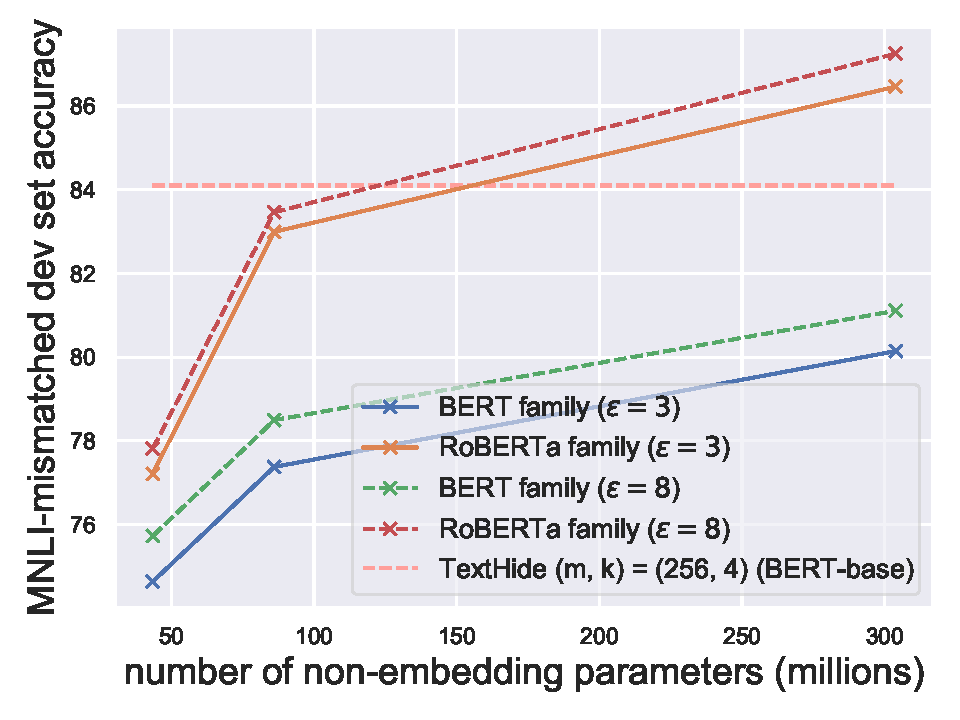
\includegraphics[width=0.98\textwidth]{figs/scaling-mnli.pdf}}
(a) MNLI-mismatched
\end{minipage}
\begin{minipage}[t]{0.45\linewidth}
\centering
{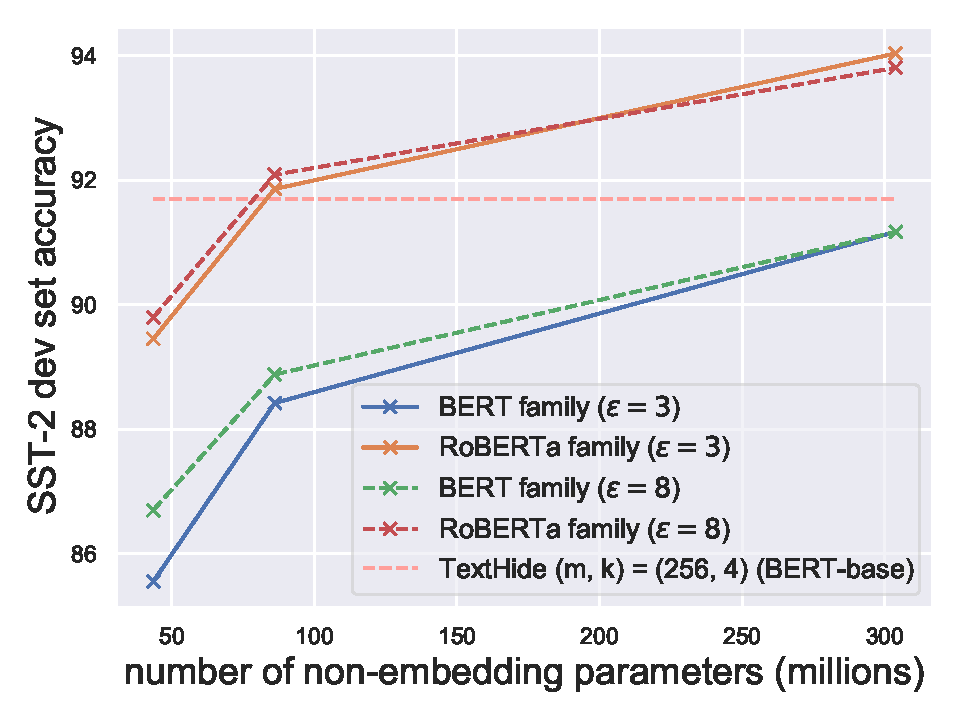
\includegraphics[width=0.98\textwidth]{figs/scaling-sst-2.pdf}}
(b) SST-2
\end{minipage}

\begin{minipage}[t]{0.45\linewidth}
\centering
{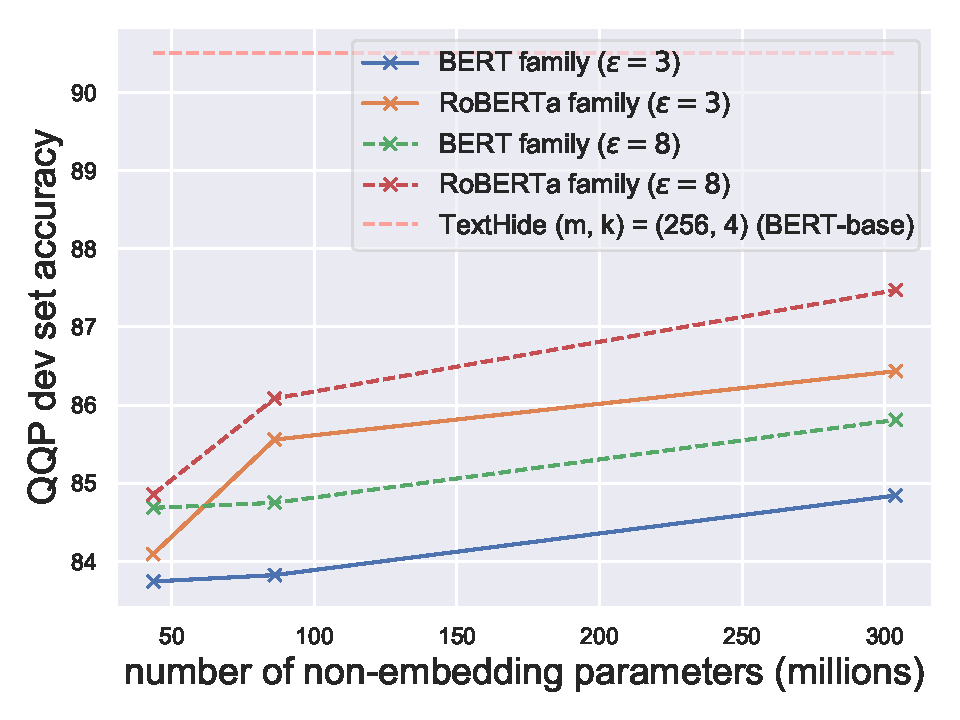
\includegraphics[width=0.98\textwidth]{figs/scaling-qqp.pdf}}
(c) QQP
\end{minipage}
\begin{minipage}[t]{0.45\linewidth}
\centering
{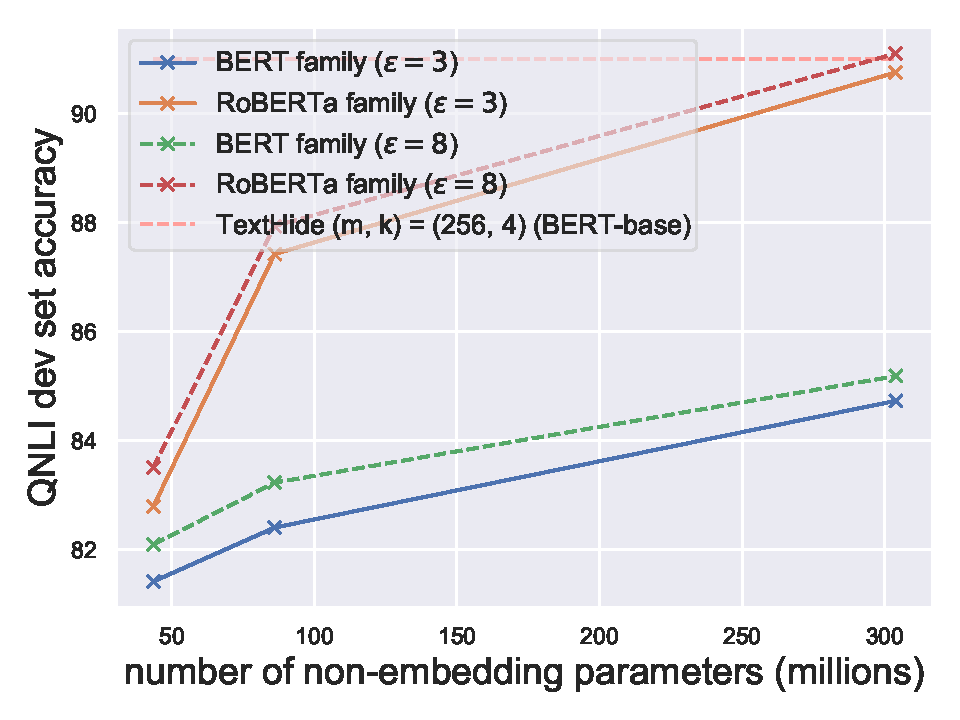
\includegraphics[width=0.98\textwidth]{figs/scaling-qnli.pdf}}
(d) QNLI
\end{minipage}
\end{center}

\begin{center}
\begin{minipage}[t]{0.45\linewidth}
\centering
{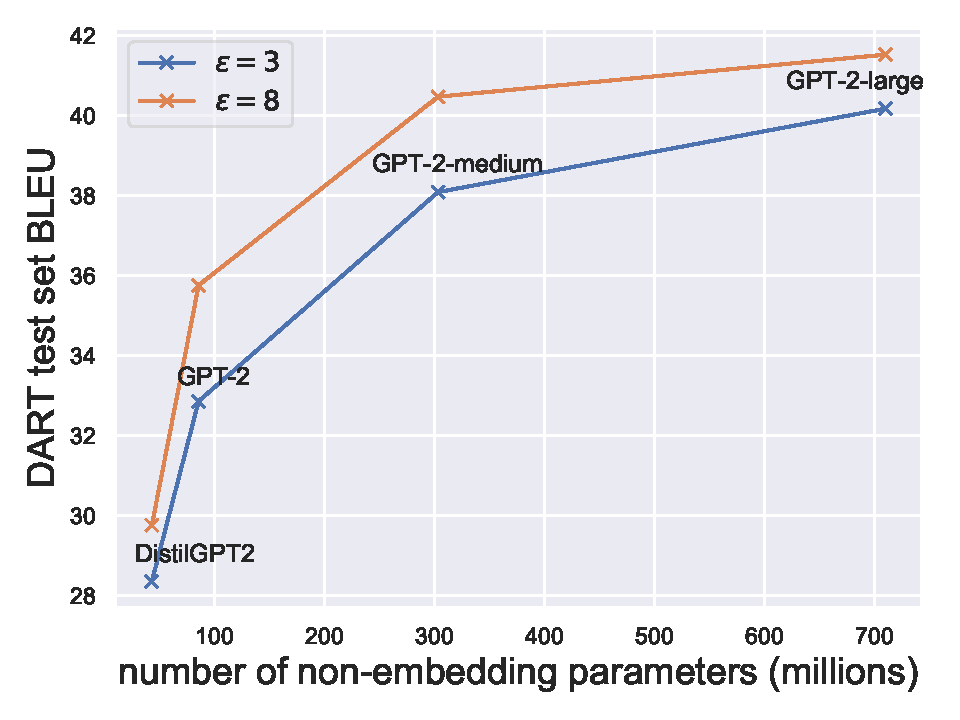
\includegraphics[width=0.98\textwidth]{figs/dart_scaling_BLEU.pdf}}
(e) DART
\end{minipage}
\end{center}

\caption{
Larger and better pretrained models consistently lead to better private fine-tuned performance on sentence classification and language generation tasks.
}
\label{fig:fig1_extension}
\end{figure}

\subsection{\normalsize Full Fine-Tuning With DP-Adam Matches State-Of-The-Art}\label{sec:experiments_main}
There is a range of lightweight fine-tuning methods that reduce the dimensionality of updates, including some that are designed for DP~\citep{yu2021large}.
Do methods that optimize fewer parameters lead to better results under DP even if they perform similarly non-privately? Empirical results suggest otherwise and that full fine-tuning is a strong baseline that even matches specialized low-dimensional DP learning methods for both classification and generation.
Below, we study the two sets of tasks separately. 
For completeness, all experimental details are in Appendix~\ref{app:experiments_main}.

\paragraph{Sentence classification.}
We study DP fine-tuning on tasks from the GLUE benchmark that have more than $10$k training examples (MNLI, QQP, QNLI, and SST-2), following the experimental setup of~\cite{yu2021large}. 
The associated datasets have modest sizes: SST-2 and QNLI have 60k+ and 100k+ training examples, respectively. MNLI and QQP each contains less than 400k examples. 
Table~\ref{table:glue} shows that using larger pretrained models and the text-infilling objective generally improve classification accuracy. 
We compare full fine-tuning with \textit{reparameterized gradient perturbation} (RGP)~\citep{yu2021large}, as it is the state-of-the-art for DP fine-tuning on sentence classification at the time the first version of this paper was uploaded to arXiv. 
The method is designed to privatize gradients projected onto low dimensional subspaces and was motivated to reduce DP noise in high-dimensional models. 
We note that full fine-tuning with the text infilling objective outperforms well-tuned RGP on all tasks despite being the simplest baseline.\footnote{The careful reader will notice that the original RGP paper~\citep{yu2021large} reported considerably worse full fine-tuning results. We analyzed their released codebase and discovered a bug caused by their use of mixed-precision training. 
With this bug fixed, their codebase produces results similar to ours for full fine-tuning on SST-2. 
We detail subtleties of DP mixed-precision training in Appendix~\ref{app:mixed_precision}, and outline our implementation which achieves approximate scale invariance.
}
Computationally, while RGP is faster per-update, it requires more than 3 times as many epochs as full fine-tuning---overall, the two methods are comparable in terms of wall time. 
\begin{table}[th]
\footnotesize
\setlength\tabcolsep{2.4pt}
\caption{
Full fine-tuning larger pretrained models  with text infilling performs best.
Results are dev set accuracies. 
Bold numbers are the best for each privacy level based on two-sample test.
$\epsilon$ estimates based on numerically composing tradeoff functions.
}
\centering
\begin{tabular}{l cccc cccc}
\toprule
\multirow{2}[2]{*}{Method} 
& \multicolumn{4}{c}{\text{$\epsilon=3$}}
& \multicolumn{4}{c}{\text{$\epsilon=8$}} \\
\cmidrule(lr){2-5}
\cmidrule(lr){6-9}
 & MNLI-(m/mm) & QQP & QNLI & SST-2
 & MNLI-(m/mm) & QQP & QNLI & SST-2 \\
\midrule
RGP {(base)} & - & - & - & - & 80.5/79.6 & 85.5 & 87.2 & 91.6 \\
RGP {(large)} & - & - & - & - & 86.1/86.0	& 86.7 & 90.0 & 93.0 \\
\midrule
full (base)              & 82.47/82.10 & 85.41 & 84.62 & 86.12 & 83.30/83.13 & 86.15 & 84.81 & 85.89 \\
full (large)             & 85.53/85.81 & \textbf{86.65} & 88.94 & 90.71 & 86.28/86.54 & \textbf{87.49} & 89.42 & 90.94 \\
full + infilling (base)  & 82.45/82.99 & 85.56 & 87.42 & 91.86 & 83.20/83.46 & 86.08 & 87.94 & 92.09 \\
full + infilling (large) & \textbf{86.43/86.46} & 86.43 & \textbf{90.76}  & \textbf{93.04} & \textbf{87.02/87.26} & 87.47 & \textbf{91.10} & \textbf{93.81} \\
\midrule \midrule
$\epsilon$ &2.75 &2.75 &2.57 &2.41 &7.15 &7.16 &6.87 &6.69\\
\bottomrule
\end{tabular}
\label{table:glue}
\end{table}



\paragraph{Table-to-text generation.}
We study different fine-tuning methods under DP for table-to-text generation where the goal is to generate natural language descriptions of table entries. 
We consider the datasets E2E~\citep{novikova2017e2e} and DART~\citep{nan2020dart}. 
E2E consists of simple restaurant reviews, whereas DART consists of open-domain table entries from Wikipedia and is more complex. 
Both datasets are small: E2E has more than 40k training examples, whereas DART has more than 60k.
Since we are the first to experiment with this task under DP, we compare full fine-tuning (full) against a suite of parameter-efficient approaches which includes LoRA~\citep{hu2021lora}, prefix-tuning~\citep{li2021prefix} (prefix), RGP, and fine-tuning the top 2 Transformer blocks (top2), all of which optimize few parameters. 
On GPT-2 (125 million parameters), prefix-tuning with default hyperparameters optimizes \mytextapprox10 million parameters; LoRA with rank 4 optimizes \mytextapprox$0.15$  million parameters. 
We also report results for training from scratch (retrain).
Hyperparameters of each method were tuned only the E2E dataset; the complete search ranges are in Appendix~\ref{app:hp_search_range}.
Table~\ref{table:e2e_trim} shows that LoRA and full fine-tuning are generally the most performant on E2E. 
% Tables~\ref{table:e2e} and \ref{table:dart} in Appendix~\ref{app:table2text} contain the full result on E2E and DART and confirm the trend.
\setlength{\tabcolsep}{2.5pt}
\renewcommand{\arraystretch}{0.75}
\begin{table}[thb]
\footnotesize
\caption{
Full fine-tuning performs on par with or outperforms others methods that execute gradient update in low dimensional spaces.
Results are on E2E from fine-tuning GPT-2.
}
\centering
\begin{tabular}{l c c c cccccc}
\toprule
\multirow{2}[0]{*}{Metric} & \multirow{2}[0]{*}{DP Guarantee} & Gaussian DP & Compose & \multicolumn{6}{c}{Method}  \\
 & & + CLT & tradeoff func. & {full} & {LoRA} & {prefix} & {RGP} & {top2} & {retrain} \\

\midrule
\multirow{3}[1]{*}{BLEU}
 & $\epsilon=3$ & $\epsilon \approx 2.68$ & $\epsilon \approx 2.75$ & \textbf{ 61.519 } & 58.153 & 47.772 & 58.482 & 25.920 & 15.457\\
 & $\epsilon=8$ & $\epsilon \approx 6.77$ & $\epsilon \approx 7.27$ & \textbf{63.189} & \textbf{ 63.389 } & 49.263 & 58.455 & 26.885 & 24.247\\
 & non-private & - & - & 69.463 & 69.682 & 68.845 & 68.328 & 65.752 & 65.731\\
\midrule
\multirow{3}[1]{*}{ROUGE-L}
 & $\epsilon=3$ & $\epsilon \approx 2.68$ & $\epsilon \approx 2.75$ & \textbf{65.670} & \textbf{ 65.773 } & 58.964 & 65.560 & 44.536 & 35.240\\
 & $\epsilon=8$ & $\epsilon \approx 6.77$ & $\epsilon \approx 7.27$ & \textbf{66.429} & \textbf{ 67.525 } & 60.730 & 65.030 & 46.421 & 39.951\\
 & non-private & - & - & 71.359 & 71.709 & 70.805 & 68.844 & 68.704 & 68.751\\
\bottomrule
\end{tabular}
\label{table:e2e_trim}
\end{table}


\paragraph{Chit-chat dialog generation.}
We stress-test full fine-tuning under DP on the task of chit-chat dialog generation. This task has the distinct challenge that the response space is intrinsically diverse~\citep{li2015diversity,gao2018neural} since human conversations can be informal and noisy~\citep{zhang2019dialogpt}.
Moreover, dialog datasets are usually formed with user data which may contain sensitive information.
We use the Persona-Chat dataset \citep{zhang2018personalizing} as a testbed and build off a processed version that has \mytextapprox{130k} training entries.
Each entry contains a dialog history, persona descriptions of the respondent, and the response. 
We fine-tune GPT-2, GPT2-medium, and DialoGPT-medium on this dataset both privately and non-privately by training to predict the response with the dialog history and persona description. 
We report the F1 score and perplexity on the validation split, and human evaluated quality scores of generations.
Table~\ref{table:personachat} shows that private models have strong performance. 
In particular, fine-tuned DialoGPT-medium at $\epsilon=8$ beats the (non-private) winning entry of the ConvAI2 challenge~\citep{dinan2019second} on perplexity and has a human evaluation rating that is close to non-private models.
Samples from our private models can be found in Appendix~\ref{app:samples}.
\begin{table}[th]
\footnotesize
\setlength\tabcolsep{2pt}
\caption{
Fine-tuning with DP-Adam yields high quality chit-chat dialog generation models. 
}
\centering
\begin{tabular}{l c c c c c c}
\toprule
\multirow{2}[0]{*}{Model} & \multirow{2}[0]{*}{DP Guarantee} & Gaussian DP & Compose & \multicolumn{3}{c}{Metrics}  \\
 & & +CLT & tradeoff func. & \scriptsize{F1} $\uparrow$  & \scriptsize{Perplexity} $\downarrow$ & \scriptsize{Quality (human)} $\uparrow$ \\
\midrule
\multirow{3}[1]{*}{GPT-2}
& $\epsilon=3$ & $\epsilon \approx 2.54$ & $\epsilon \approx 2.73$ & 15.90 & 24.59  & - \\
& $\epsilon=8$ & $\epsilon \approx 6.00$ & $\epsilon \approx 7.13$ & 16.08 & 23.57  & - \\
& non-private  & - & - & 17.96 & 18.52  & - \\
\midrule
\multirow{3}[1]{*}{GPT-2-medium}
& $\epsilon=3$ & $\epsilon \approx 2.54$ & $\epsilon \approx 2.73$ & 15.99 & 20.68  & - \\
& $\epsilon=8$ & $\epsilon \approx 6.00$ & $\epsilon \approx 7.13$ & 16.53 & 19.25  & - \\
& non-private &- &- & 18.64 & 15.40  & - \\
\midrule
\multirow{3}[1]{*}{DialoGPT-medium}
& $\epsilon=3$ & $\epsilon\approx 2.54$ & $\epsilon \approx 2.73$ & \textbf{17.37} & \textbf{17.64}  & 2.82 (2.56, 3.09)\\
& $\epsilon=8$ & $\epsilon\approx 6.00$ & $\epsilon \approx 7.13$ & \textbf{17.56} & \textbf{16.79}  & 3.09 (2.83, 3.35)\\
& non-private &- &- & 19.28 & 14.28  & 3.26 (3.00, 3.51)\\
\midrule
HuggingFace {\scriptsize (ConvAI2 winner)} & non-private &-	&- & 19.09 & 17.51 & - \\
HuggingFace {\scriptsize (our implementation)} & non-private &- &- & 16.36 & 20.55 & 3.23 (2.98, 3.49) \\
\midrule
Reference &- &- &- &- &- & 3.74 (3.49, 4.00) \\
\bottomrule
\end{tabular}
\label{table:personachat}
\end{table}


